
\section{PC Cluster: Design and Implementation}
\label{sec:implementation}

Thus far, we have mostly considered lower-level systems issues (the design and implementation of the PC object mode, TCAP optimization and vectorized processing) and
the programming interface that PC offers to end-users.  In this section, we discuss how these pieces fit together into the PC System at large.  First we 
describe PC's overall architecture, and then we detail how all of these pieces work together to process distributed aggregations and distributed joins.

\subsection{System Architecture}

The overall PC system architecture is illustrated in Figure~\ref{fig:arch}.
A PC cluster consists of a \emph{master node} as well as one or more \emph{worker nodes}.
The master node runs a \emph{master server}, which consists of
four software components: 

\begin{figure}
\centering
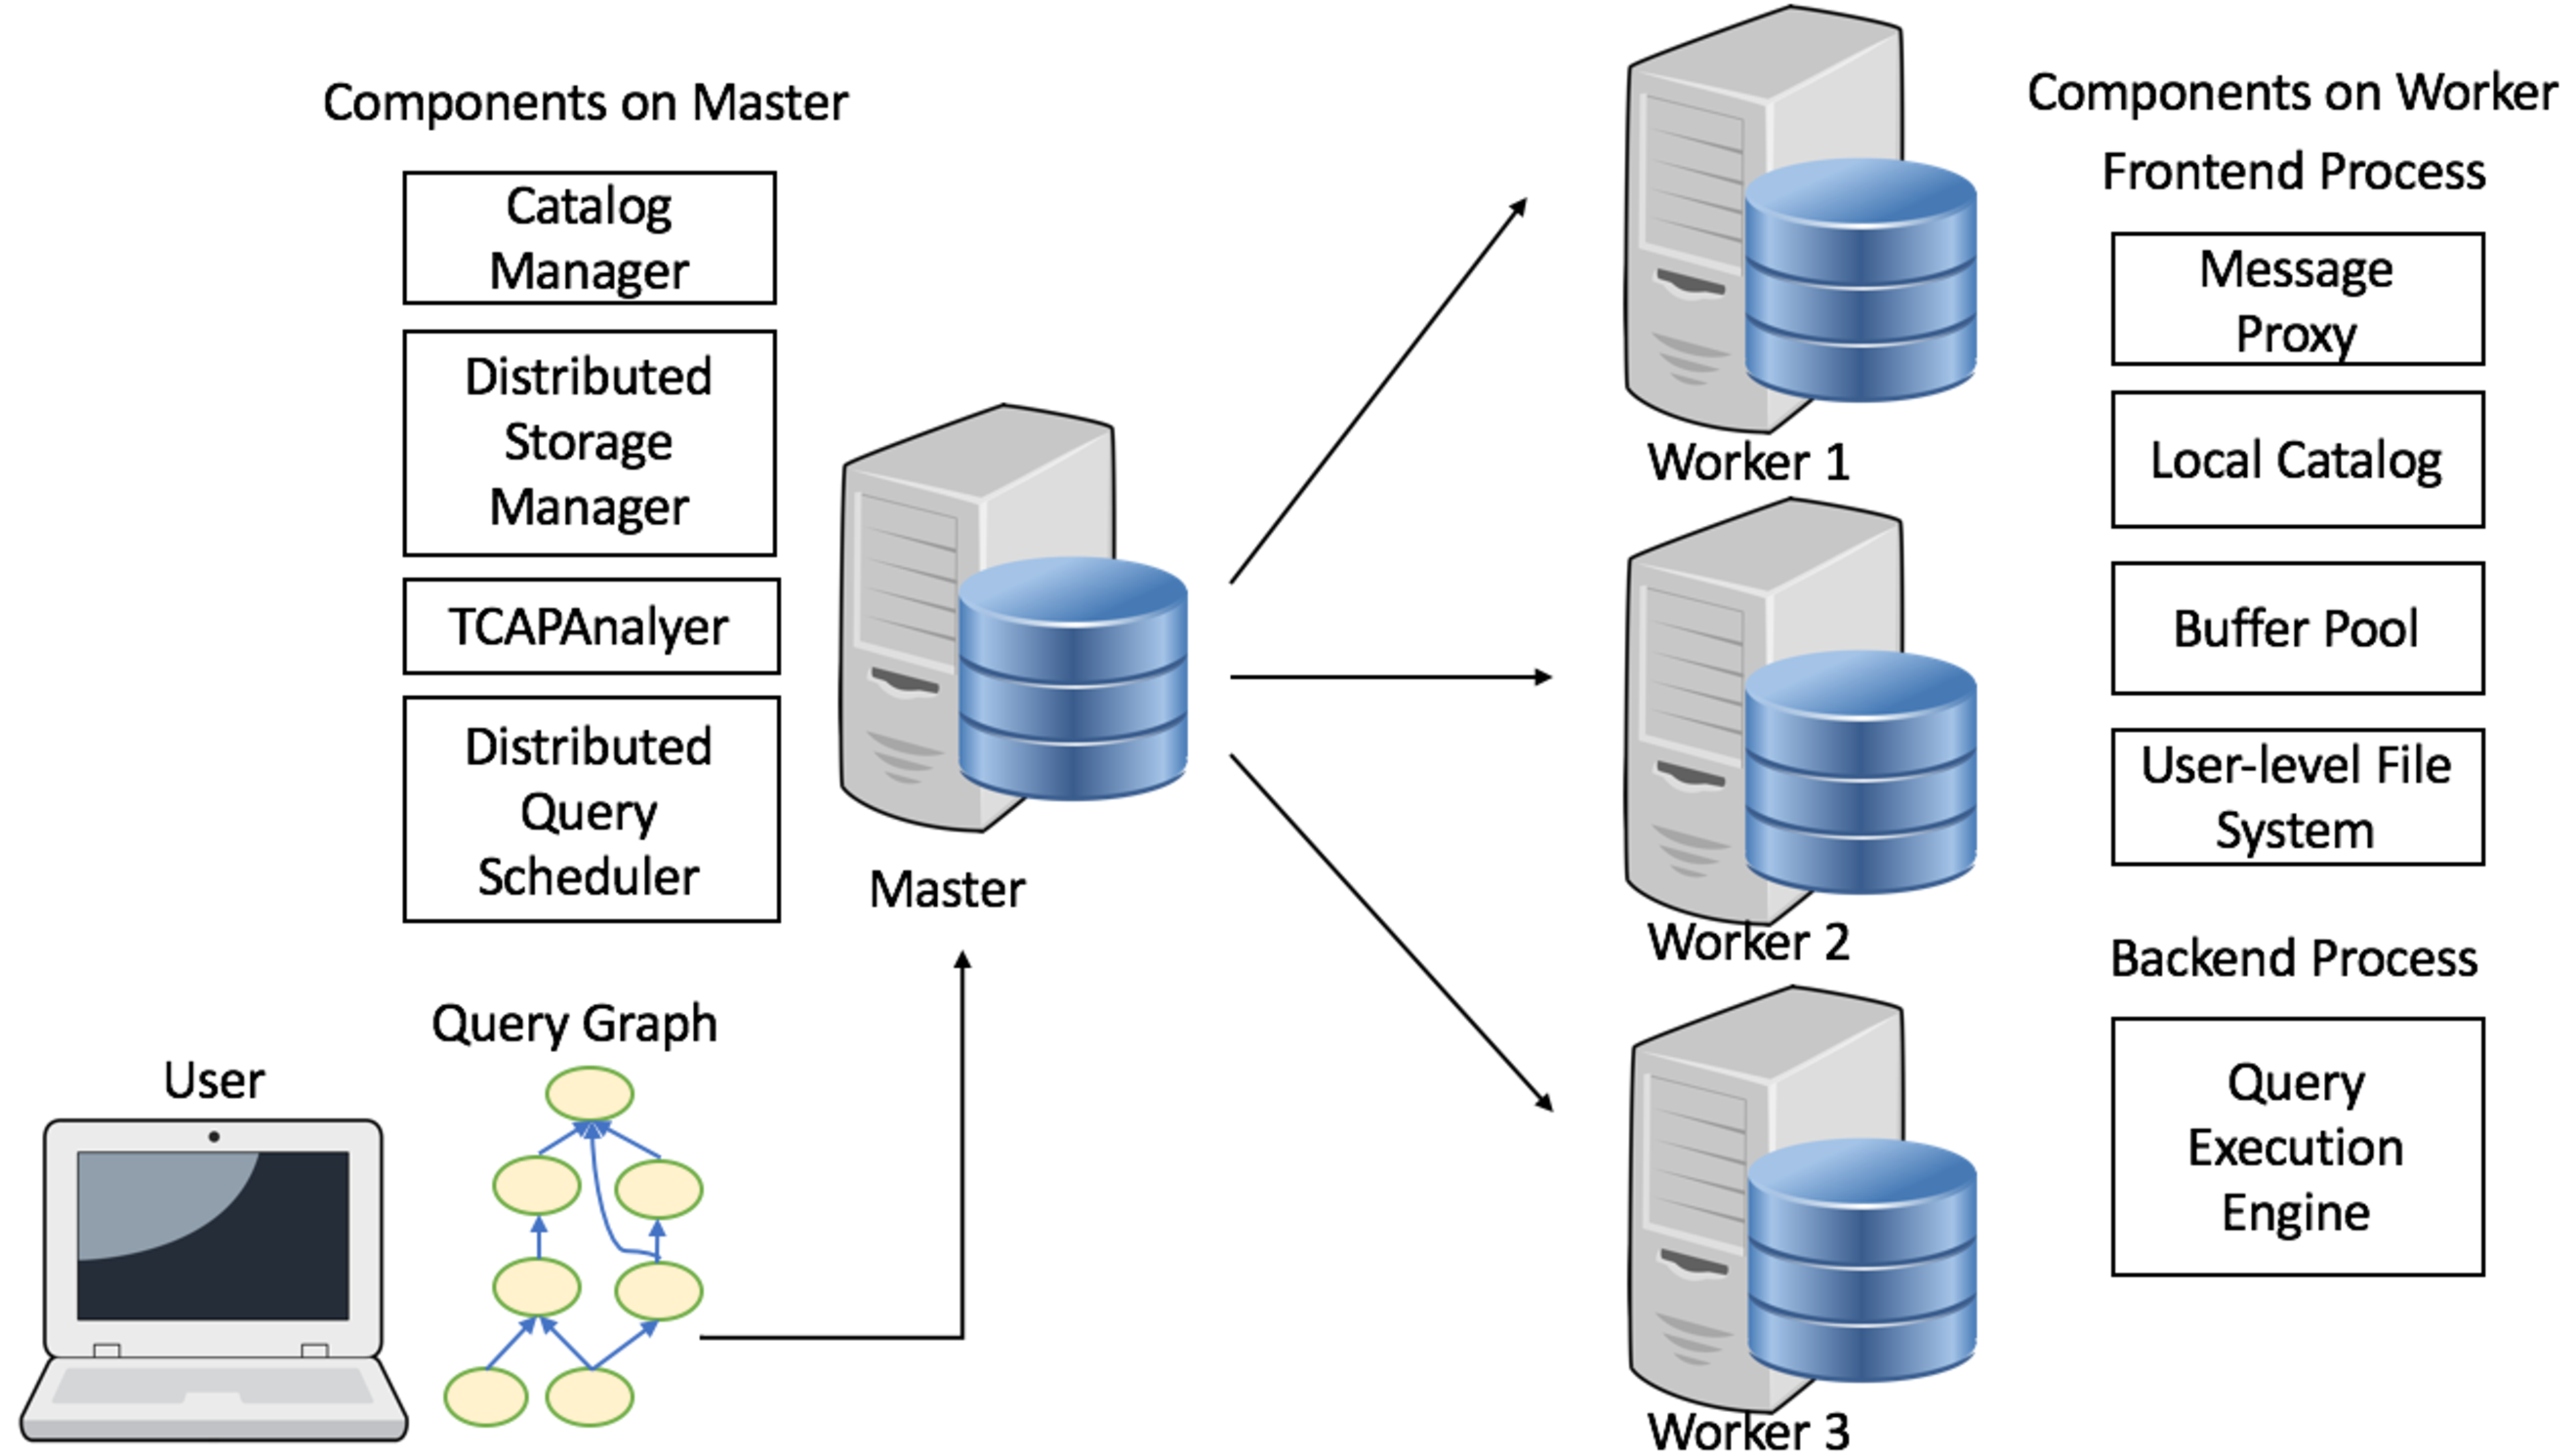
\includegraphics[width=0.75\textwidth]{arch.pdf}
  \caption{\label{fig:arch} PC distributed runtime.}
\end{figure}


\begin{enumerate}
\item The \emph{catalog manager}, serving system meta-data (including the master copy of
the mapping between type codes and PC \texttt{Object} types) and compiled, shared libraries
for performing computations over PC \texttt{Object}s;
\item The \emph{distributed storage manager}, 
the centralized server that manages PC's storage subsystem; 
\item The \emph{TCAP optimizer} which is responsible for optimizing
  programs that have been compiled into PC's domain-specific TCAP
  language (as in 
Section \ref{sec:optimizer} of the paper);
\item The \emph{distributed query scheduler} that is responsible for accepting optimized TCAP computations.
It dynamically transforms those computations into a set of JobStages,
such as:
\texttt{PipelineJobStage}, which consists of a series of pipeline stages as
described in Section~\ref{sec:pipelined} in the paper;
\texttt{AggregationJob Stage}, to perform aggregation on shuffled data that is
generated by a PipelineJobStage; and \texttt{Build HashTableJobStage}, to build hash
tables using shuffled data or broadcasted data that is generated by a
PipelineJobStage. Then it
dynamically schedules those job stages as well as initiates and
monitors execution of the job stages on the cluster.
\end{enumerate}

\noindent 
Each worker node in a PC cluster runs two processes: the \emph{worker front-end process} and the \emph{worker backend process}.
Dual processes are used because PC executes potentially unsafe native user code.  By definition, user code is run only in the backend process so that the
worker front-end process is ``crash proof''---if            
user code happens to crash the worker backend process, the worker front-end process will receive a signal and it can re-fork the worker
backend process.

The worker front-end process runs following components:

\begin{enumerate}
\item The \emph{local catalog manager} that requests and 
buffers data served from the master server's catalog manager.  The local catalog manager is also responsible for fetching and dynamically loading
code as needed when a virtual method call is made over a PC \texttt{Object} (see Section \ref{sec:dyn_dis} of the paper);
\item The \emph{storage server}, a local storage server that manages a shared-memory buffer pool used for buffering and caching datasets.  It also manages
a  user-level file system that is used to persist a portion of one or more data sets stored by PC (the partitioning of data sets to storage servers is managed
by the master server's distributed storage manager).  The storage server also manages temporary data that must be spilled to secondary storage.
The shared memory buffer pool is created via a \texttt{mmap} system call so that
data stored in it can be read by the backend process (forked from
the frontend process) via zero-copy access;
\item And finally, the \emph{message proxy} which is responsible for communicating the with the worker backend process, and which acts as a bridge between the
worker backend process and the master server, the local catalog, and the local storage server.

\end{enumerate}

Because worker backend processes are the only processes that are actually allowed to run user code (and because user code is that code that actually processes
user-supplied data) it means that the worker backend processes are
where all computations in PC are actually performed.  A computation in PC corresponds either
to execution of the 
JobStages such as \texttt{PipelineJobStage}, \texttt{AggregationJobStage},
\texttt{BuildHashTableJobStage}, that are created by the master server's distributed query scheduler, 
or of executing the computations and required communications
that link together the various JobStages to implement distributed computations such as joins and aggregations.  

In the next two subsections, we describe how PC implements two of its distributed computations: distributed aggregation, and a distributed hash-partition join.

\subsection{Distributed Aggregation}

The workflow of PC's distributed aggregation implementation is
shown in Figure ~\ref{fig:aggregation}.
The most unique aspect of distributed aggregation in PC is the way in which it is tightly coupled with the PC \texttt{Object} model.  All data structures used
to power distributed aggregation are themselves PC \texttt{Objects}, and hence they all provide for zero-cost data movement, avoiding
serialization and deserialization overhead when shuffling data.

Distributed aggregation in PC is broken into two different job stages.
In the first, there is a \texttt{PipelineJobStage} working as a \emph{producing stage},
where all required pre-aggregation computations are performed, and then the
data are pre-aggregated and stored in a set of hash tables (that is, PC \texttt{Map} objects).  These PC \texttt{Map} objects are shuffled, so that all partial aggregates
associated with the same key are on the same machine.  Then in a
second job stage, which is a \texttt{AggregationJobStage} working as the \emph{consuming stage},
the shuffled \texttt{Map} objects from around the cluster are then aggregated
to produce the final aggregation result.

\begin{figure}
\centering
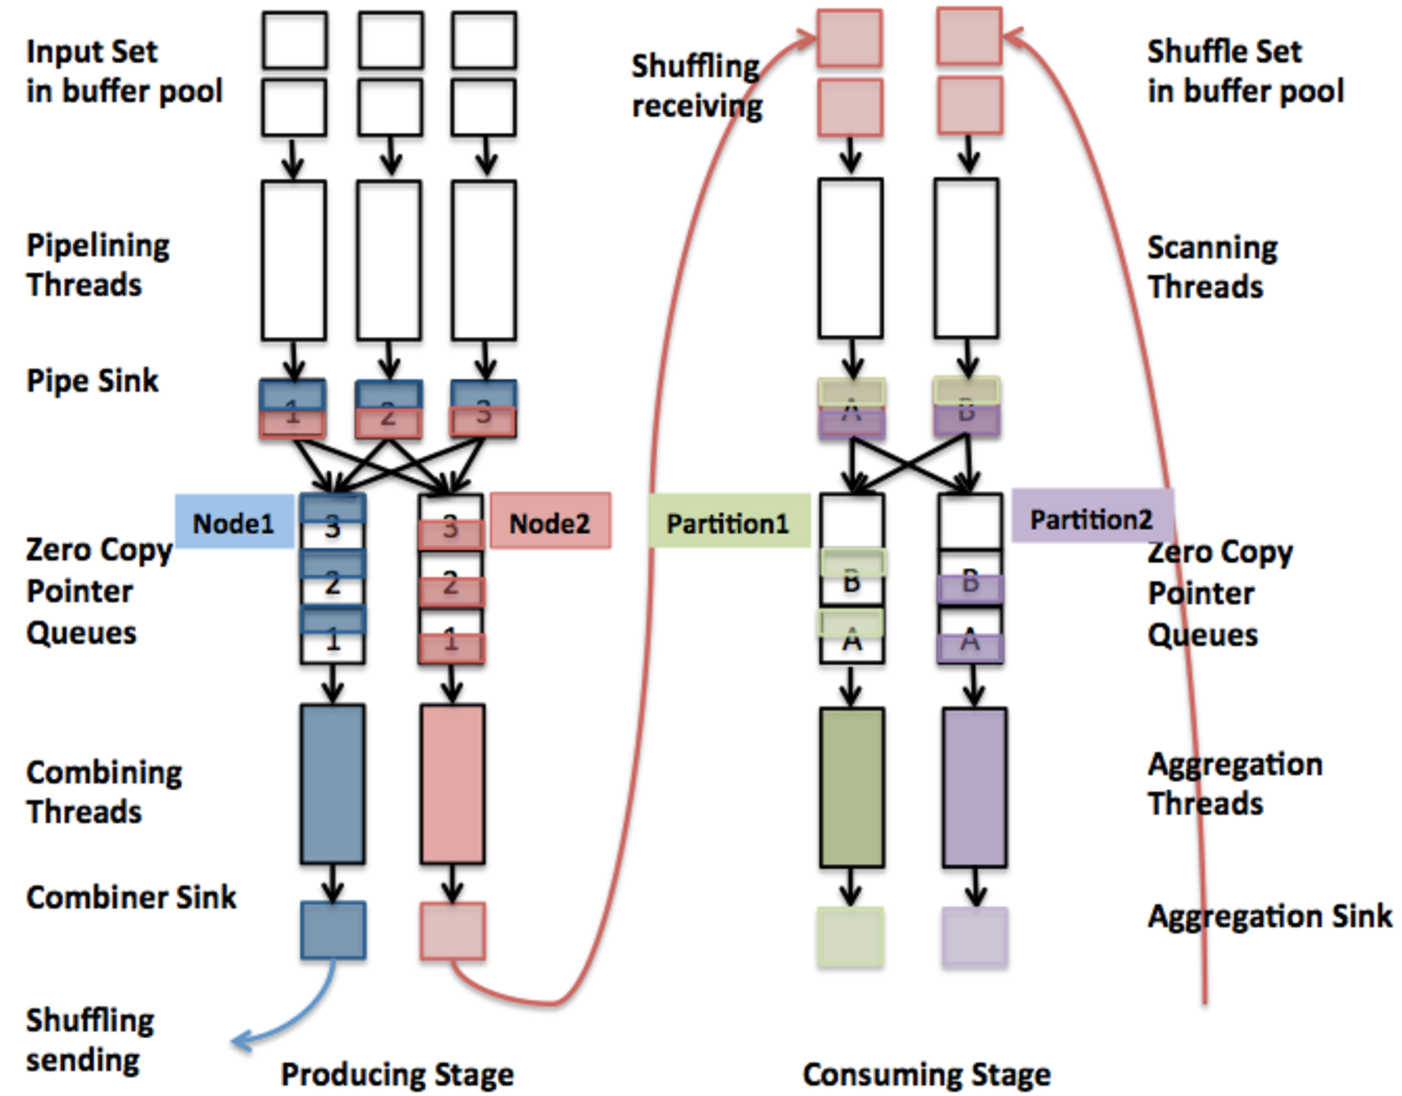
\includegraphics[width=0.75\textwidth]{aggregation.pdf}
  \caption{\label{fig:aggregation} Distributed aggregation in PC.}
\end{figure}

\vspace{5pt}
{\bf 1. The producing stage.} In this stage, a sequence of TCAP operations that end in an \texttt{AGGREGATE} operation are used to create a pipelined job stage which is 
realized as a list
of pipelined stages, where each stage corresponds to a TCAP operation.
A replica of the list of pipelined stages is
created for each of the $N$ so-called \emph{pipelining threads} dedicated to implementing
the producing stage on each of the backend worker processes.  
The thread assigned to each of those pipelines begins by allocating a PC \texttt{Vector <Handle <Map <Object, Object>>} on an output page.  This page will serve
as the \emph{pipe sink}.  The pipe sink is
the location where the data produced by the pipeline are stored.  In this way the PC \texttt{Object} model is used to store the results
from the producing stage, so that they can be sent over the network and used at the other side with no serialization/deserialization.

Once the pipe sinks have been allocated,
the system begins assigning input pages to each of the pipelining 
threads.  Each input page was itself produced as a the result of a previous pipelined job stage, or else has been
loaded from storage.  Hence all pages are themselves organized using the PC \texttt{Object} model.  Thus, each input
page will itself contain a \texttt{Vector <Handle <Object>>},
or another standard PC container type.  During the producing stage, vectors of PC \texttt{Handle}s are repeatedly
loaded from each input page, and each is used to create a vector list that is pushed through the list of pipeline stages.

Ultimately, pushing a vector list through the pipeline stages results in an output vector list that contains a vector of keys and a vector of values 
associated with those keys that need to be aggregated.  
For each (key, value)
pair, first the key is hashed to a particular \emph{hash partition}---the hash partition determines which of the \texttt{Map}
objects in the \texttt{Vector <Handle <Map <Object, Object>>} stored on the output page will receive the pair, and which machine will house the final aggregation
for all instances of the key.  Once the hash partition has been determined,
the pair is added to the associated \texttt{Map} in the pipe sink
(if a particular key is already there, the
existing value is added to the new value, and the result is used to replace the existing value).  

At the same time, 
$K$ different \emph{combining threads} are running in each backend worker process.  
When a page containing a \texttt{Vector <Handle <Map <Object, Object>>} becomes full, the thread running the associated pipeline stage allocates a new
pipe sink,
and the filled page is added to the queue of completed pages to be processed.  There is one such queue
associated with each of the $K$ combining threads.
We call each such queue a \emph{zero copy pointer queue} because the entire page of PC \texttt{Object}s is passed from a pipelining thread to each of the
combining threads as a pointer, with no PC \texttt{Object} movement.

Each combining thread is assigned one or more hash partitions.  When a combining thread
is a associated with a hash partition, it is responsible for 
aggregating all of the \texttt{Map}s produced by local pipelining threads that were associated with that hash partition.
The result is a 
\texttt{Map} containing data for that one hash partition.  Since each combining
thread can be assigned more than one hash partition that will be sent to the same destination machine,
the combining thread also produces a \texttt{Vector <Handle <Map <Object, Object>>} that is referred to as a \emph{combining sink}.
Each \texttt{Map} in the \texttt{Vector} is associated with one hash partition.
This object is stored on a thread-local \emph{combiner page} whose size is automatically tuned by the system.

\vspace{5pt}
{\bf 2. The consuming Stage.}
Once a combiner page becomes full, the page is directly sent to the worker node housing the
backend worker processes tasked with processing the set of hash partitions on the page.
This communication is referred to as a \emph{shuffle}.  
Compression is used to reduce the shuffle data size and save on network cost.
When a worker node receives a page during the shuffle, one of a pool of \emph{scanning threads} will look at the 
\texttt{Vector <Handle <Map <Object, Object>>} object contained in the page, and then add a pointer to the page
to the each of the queues associated with the $M$ \emph{aggregation threads}.  These are the threads
that are tasked with final processing of all of the various hash partitions.
Each aggregation thread is responsible for aggregating exactly 
one hash partition, and so $M$ is the total number of hash partitions processed by a given backend worker process.
An aggregation thread has an output page housing its \emph{aggregation sink}.  The aggregation sink is a \texttt{Map <Object, Object>} that stores the portion of the
data that it aggregates.

 
In PC, all of the ``magic'' parameters such as the number of hash partitions $M$, 
the number of pipelining threads $N$, 
the number of combining threads for each remote node $K$, 
the combiner page size, and the aggregation page size are all automatically 
determined at run-time to maximize memory utilization, network utilization and CPU utilization. 

\subsection{Hash Partition Join}

We now briefly describe how PC implements a distributed equi-join of $n$ different sets using a hash-partition strategy.  
That is, imagine that $t$ = $\langle t_1, t_2, ..., t_n \rangle$ is a
tuple formed by taking one item from each of the $n$ sets.  Let $key(t_i)$ denote the join key of $t_i$.  Then an $n$-way equi-join requires that
in order for $t$ to be in the output set, it must be the case that
$key(t_i) = key(t_j)$ forall $i, j$. 

In PC, such an operation is broken into $2n$ job stages. The first $n$ job stages repartition each of the $n$ sets, so that all of the data with the same join key value
must be co-located on the same machine.  The next $n - 1$ job stages hash all of the entries in $n - 1$ of those sets.  The last job stage scans the last set and
probes the constructed hash tables.  

In more detail, the three types of job stages are:

\vspace{5pt}
{\bf 1. The data repartition job stages.} This class of job stage is similar to the producing stage in distributed
aggregation, with one key difference.
Rather than using a \texttt{Vector <Handle <Map <Object, Object>>>} to store (key, value) pairs where the value is the result obtained by aggregating a set of
data with the same key, the pipe sink used is instead a \texttt{Vector <Handle <Map <unsigned\_t, Vector <Object>>>>} data structure.  Here, the
\texttt{unsigned\_t} is a hash value produced by a TCAP \texttt{HASH} operation over the input object's join key, and the \texttt{Vector <Object>} is a list of objects
with the same hash value.  
When a new object with the same hash key is found during pipelined processing or during combining, rather than aggregating, the new object is instead inserted
into the inner \texttt{Vector <Object>} data structure that contains a set of objects with the same hash key.
Note that after the data repartition job stages completes, all of the data from all of the sets will have been repartitioned, so that all of the data with the same join
key will be co-located on the same machine.

\vspace{5pt}
{\bf 2. The hash table building job stages.} These job stages are similar to the consuming job stage in aggregation, 
except that again, rather than aggregating, the goal is to build up \texttt{Vector}s of objects, stored in various \texttt{Map} data structures (one for each
aggregation thread), where the \texttt{Vector} of objects associated with a particular 
\texttt{unsigned\_t} contains \emph{all} of the objects in a set whose join key hashes to that particular \texttt{unsigned\_t} value.
As a reult of this class of job stage, the contents of $n - 1$ of the input sets will be stored precisely as required.

\vspace{5pt}
{\bf 3. The hash join job stage.} 
This job stage is also analogous to the consuming job stage in aggregation, but the hash join job stage is run over the last set (the one that was not 
hashed as part of join stage 2). Now imagine that we are processing the last data set, after shuffling.  At this point,
all of the other sets have been
stored in \texttt{Map <unsigned\_t, Vector <Object>>} objects.  As we process the final set,
the hash value for each ofject is used to probe the \texttt{Map}
associated with each of the other $n-1$ sets.  If a match is found in each one of those other $n-1$ sets, then
one or more entries in the output vector list are created to store the matches.  The resulting vector sets are then pushed through a pipeline that post-processes
the data in the vector list, likely checking to see if this was an actual match (and not just an accidental hash collision) and perhaps performing the processing
necessary to prepare for the \emph{next} join or aggregation.
Note that if $m_i$ objects from the $i$th input set have the same \texttt{unsigned\_t} hash value, then $\prod_i m_i$ entries in a vector set will be created
as a result of these hash table probes. 

%\subsection{Dynamic Query Scheduling}
%Now we briefly describe the implementation of dynamic scheduling of job stages. 
%
%A TCAP compiler compiles the TCAP automatically coded from user query graph into a query plan that is a graph connecting TCAP instructions with native code generated for executing each instruction. 
%
%Then the TCAP analyzer will search the query graph to look for the best job stage to execute, based on a cost model that considers size of source sets, size of sink set and data locality. The goal is to minimize generated intermediate data size,  and in the same time to execute all computations that are related with one dataset as close as possible to improve memory locality and avoid unnecessary data eviction from memory.
%
%%%Once the optimal job stage is identified, the distributed query scheduler will allocate datasets through the distributed storage manager, schedule the stage to run across the cluster, collect the statistics such as the size of result datasets, and remove unused datasets. Then based on the updated statistics, a new job stage will be identified as the optimal one and get scheduled until the query plan has been fully executed.
